% !TEX root = ../PRACA_MAIN.tex
\section{Porównanie algorytmów rekomendacyjnych}

W niniejszym rozdziale przeprowadzono ewaluację i porównanie skuteczności wybranych algorytmów rekomendacyjnych. Głównym celem badań było zestawienie ze sobą modeli reprezentujących trzy różne paradygmaty: klasyczną faktoryzację macierzy (BPR), głębokie sieci neuronowe (NCF) oraz grafowe sieci neuronowe (LightGCN).

Rozdział został podzielony na trzy główne sekcje. W pierwszej z nich szczegółowo opisano proces doboru i optymalizacji hiperparametrów, mający na celu maksymalizację zdolności predykcyjnych każdego z modeli. W kolejnej części zestawiono wyniki eksperymentów przeprowadzonych na zbiorze danych MovieLens i poddano je analizie pod kątem przyjętych metryk oceny (m.in. NDCG oraz Recall). Rozdział kończy dyskusja uzyskanych wyników oraz wnioski dotyczące skuteczności i ograniczeń badanych architektur w zadaniu rekomendacji Top-N.

\subsection{Proces strojenia hiperparametrów}

W celu uzyskania stosunkowo najlepszych możliwych wyników badanie poprzedzono procesem doboru odpowiednich hiperparametrów. Przyjęto następującą metodologię. W pierwszej kolejności zbadano poziom wrażliwości algorytmów na zmiany wartości określonych parametrów. Następnie bazując na wynikach zdefiniowano okrojoną siatkę hiperparametrów dla każdej z metod i przy pomocy metody Grid Search polegającej na zbadaniu wszystkich możliwych kombinacji określonych wcześniej wartości wyłoniono najlepsze zestawy parametrów będące podstawą późniejszej analizy porównawczej.

Dobór parametrów poddanych analizie wrażliwości wynikał z ich kluczowego wpływu na zdolności predykcyjne oraz charakterystyki architektonicznej każdego z badanych algorytmów:
\begin{itemize}
    \item W modelu \textbf{ItemKNN} wybrano rozmiar sąsiedztwa ($k$) oraz współczynnik wygładzania (ang. \foreignlanguage{english}{\textit{shrinkage}}). Parametr $k$ determinuje, na ilu najbardziej podobnych elementach bazuje predykcja, co jest kluczowe w filtrowaniu opartym na sąsiedztwie. Współczynnik wygładzania pozwala z kolei na redukcję szumu statystycznego przy obliczaniu podobieństwa dla rzadko ocenianych przedmiotów.
    \item Dla modelu \textbf{BPR} skupiono się na współczynniku uczenia (ang. \foreignlanguage{english}{\textit{learning rate}}) oraz rozmiarze wektora cech ukrytych (ang. \foreignlanguage{english}{\textit{embedding size}}). Współczynnik uczenia determinuje zbieżność optymalizacji. Z kolei złożoność faktoryzacji macierzy rośnie wraz z wymiarem przestrzeni latentnej, dlatego optymalizacja tego parametru jest kluczowa dla balansu pomiędzy niedouczeniem a przeuczeniem.
    \item W głębokim modelu \textbf{NeuMF} analizie poddano współczynnik uczenia oraz prawdopodobieństwo odrzucenia neuronów (ang. \foreignlanguage{english}{\textit{dropout probability}}). Głębokie sieci neuronowe są wysoce podatne na zapamiętywanie danych treningowych (ang. \foreignlanguage{english}{\textit{overfitting}}), dlatego właściwy dobór parametru dropout jest niezbędny do uzyskania dobrej zdolności do generalizacji.
    \item W przypadku grafowego modelu \textbf{LightGCN} wytypowano wagę regularyzacji (ang. \foreignlanguage{english}{\textit{regularization weight}}) oraz liczbę warstw propagacji (ang. \foreignlanguage{english}{\textit{number of layers}}). Regularyzacja L2 kontroluje wielkość wag wektorów zapobiegając nadmiernemu dopasowaniu, podczas gdy liczba warstw odpowiada za eksplorację sygnałów wyższego rzędu w grafie (np. odległości 2-skokowe).
\end{itemize}

\subsubsection{Analiza wrażliwości}

Poniżej przedstawiono graficzne zestawienie wpływu badanych hiperparametrów na metrykę NDCG@10 dla każdego z algorytmów.
W przypadku modelu ItemKNN (Rysunek \ref{fig:sweep_itemknn}) można zaobserwować, że zwiększanie liczby uwzględnianych sąsiadów ($k$) konsekwentnie poprawia wyniki metryki NDCG@10 aż do wartości $k=200$, po czym przyrost ten naturalnie zwalnia. Regularyzacja \textit{shrinkage} z kolei nie przynosi w tym przypadku znaczących korzyści na zbiorze MovieLens 100K -- najwyższy wynik odnotowano dla braku wygładzania (wartość 0.0), a dalsze zwiększanie tego parametru skutkuje delikatnym i marginalnym spadkiem trafności.

\begin{figure}[H]
    \centering
    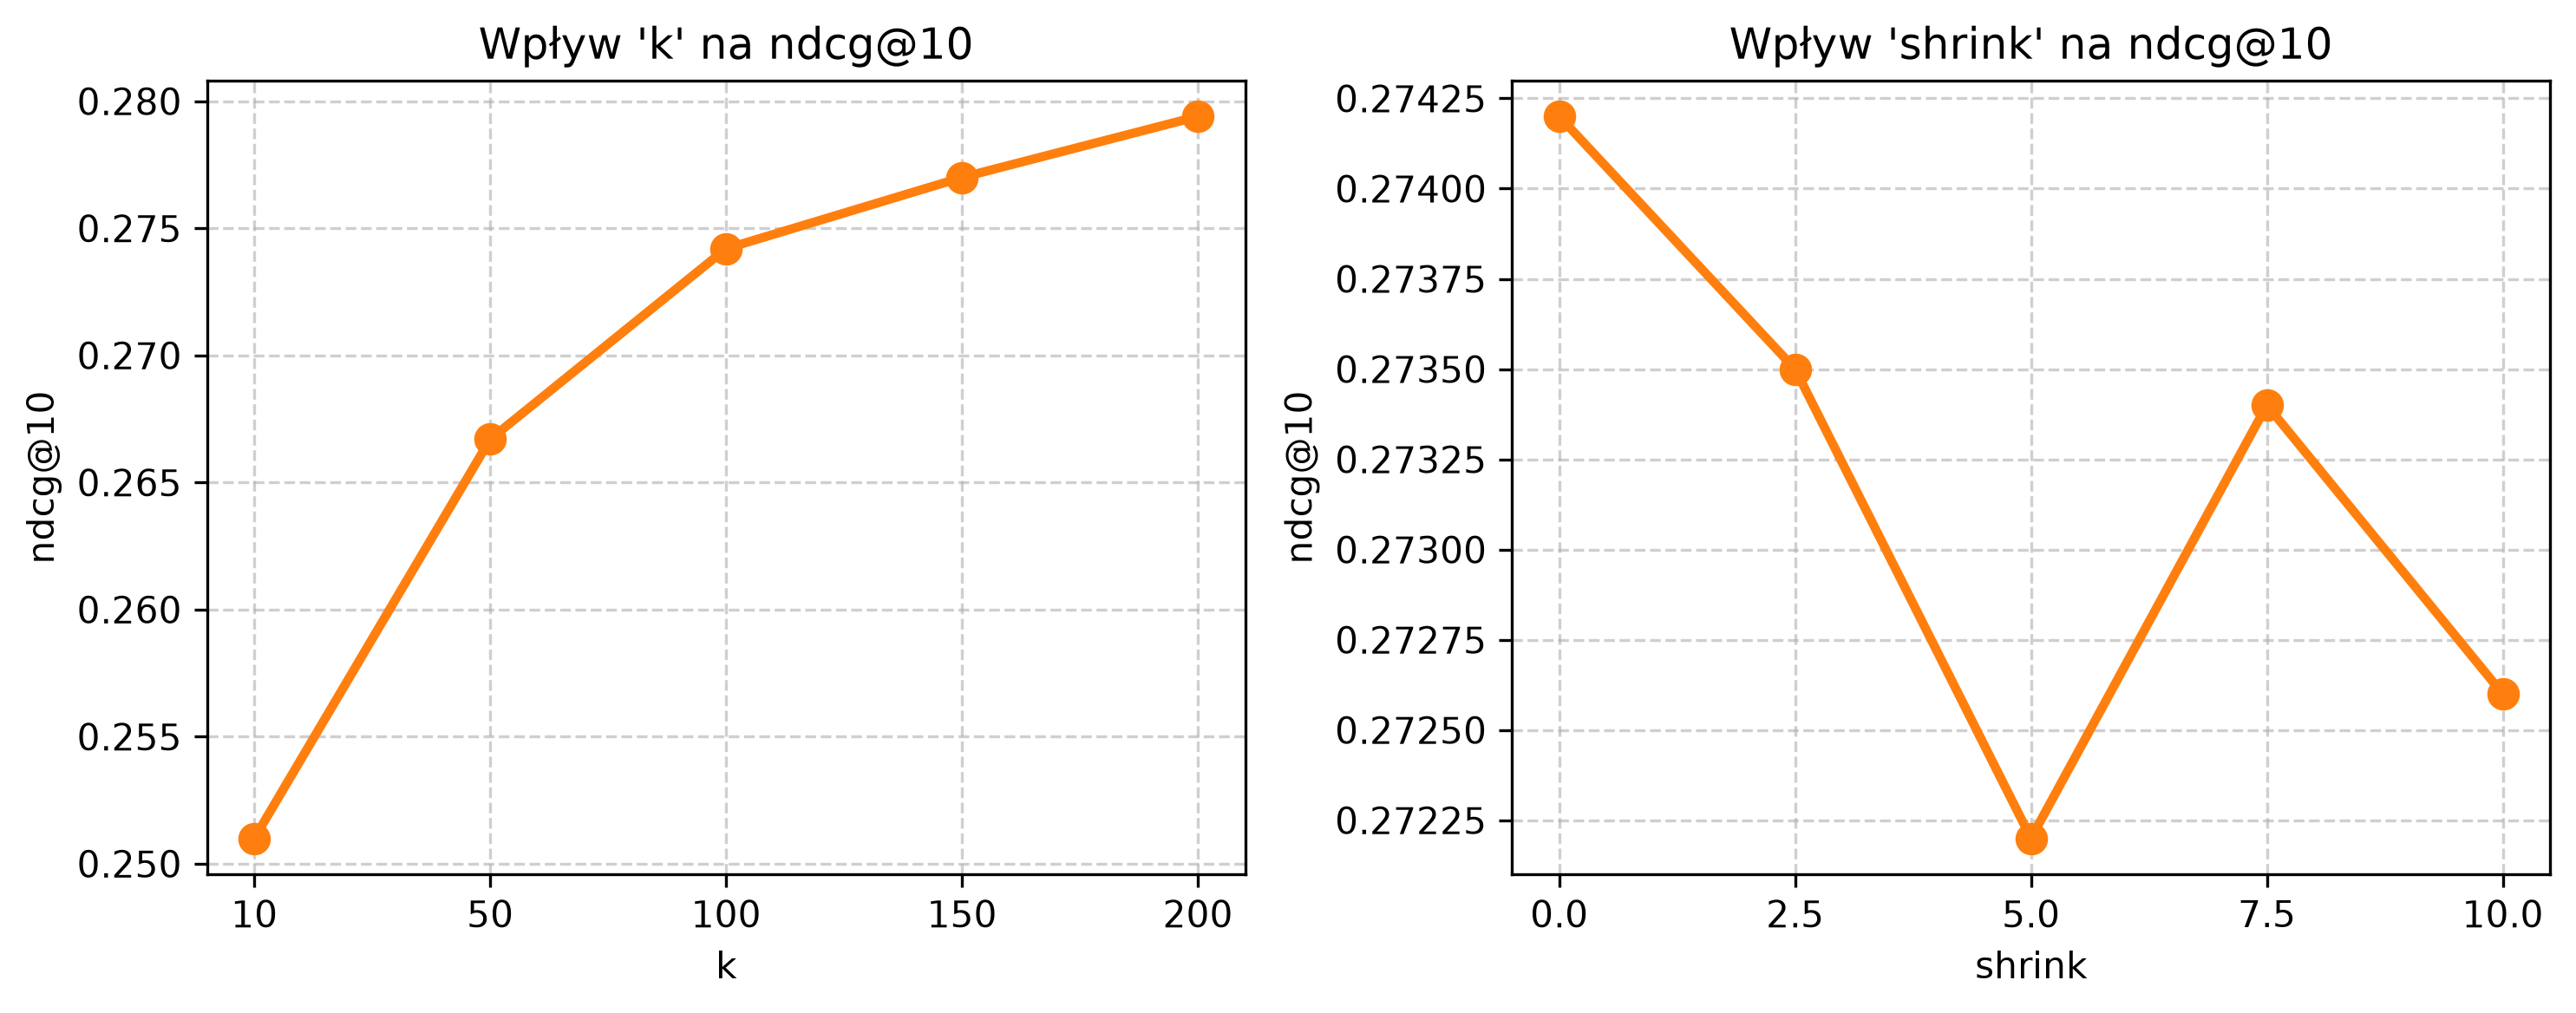
\includegraphics[width=\textwidth]{img/sweep_itemknn_summary.png}
    \caption{Wpływ hiperparametrów $k$ oraz \textit{shrinkage} na trafność modelu ItemKNN}
    \label{fig:sweep_itemknn}
    \vspace{0.2cm}\noindent{\raggedright \small \textbf{Źródło:} opracowanie własne.\par}
\end{figure}

Dla modelu faktoryzacji BPR (Rysunek \ref{fig:sweep_bpr}) analiza ujawnia klasyczną zależność optymalizacyjną. Współczynnik uczenia osiąga jednoznaczne optimum na poziomie 0.0005, zapewniając najwyższą trafność na poziomie NDCG@10 $\approx$ 0.2867. Większe wartości prowadzą do spadku trafności w wyniku niestabilności numerycznej. Z kolei rozmiar wektora cech wskazuje, że wartość 128 oferuje optymalną celność (niewielka przewaga nad 64), podczas gdy dalsze zwiększanie do wymiaru 256 skutkuje spadkiem skuteczności spowodowanym powolnym przeuczaniem się algorytmu na treningowej części zbioru.

\begin{figure}[H]
    \centering
    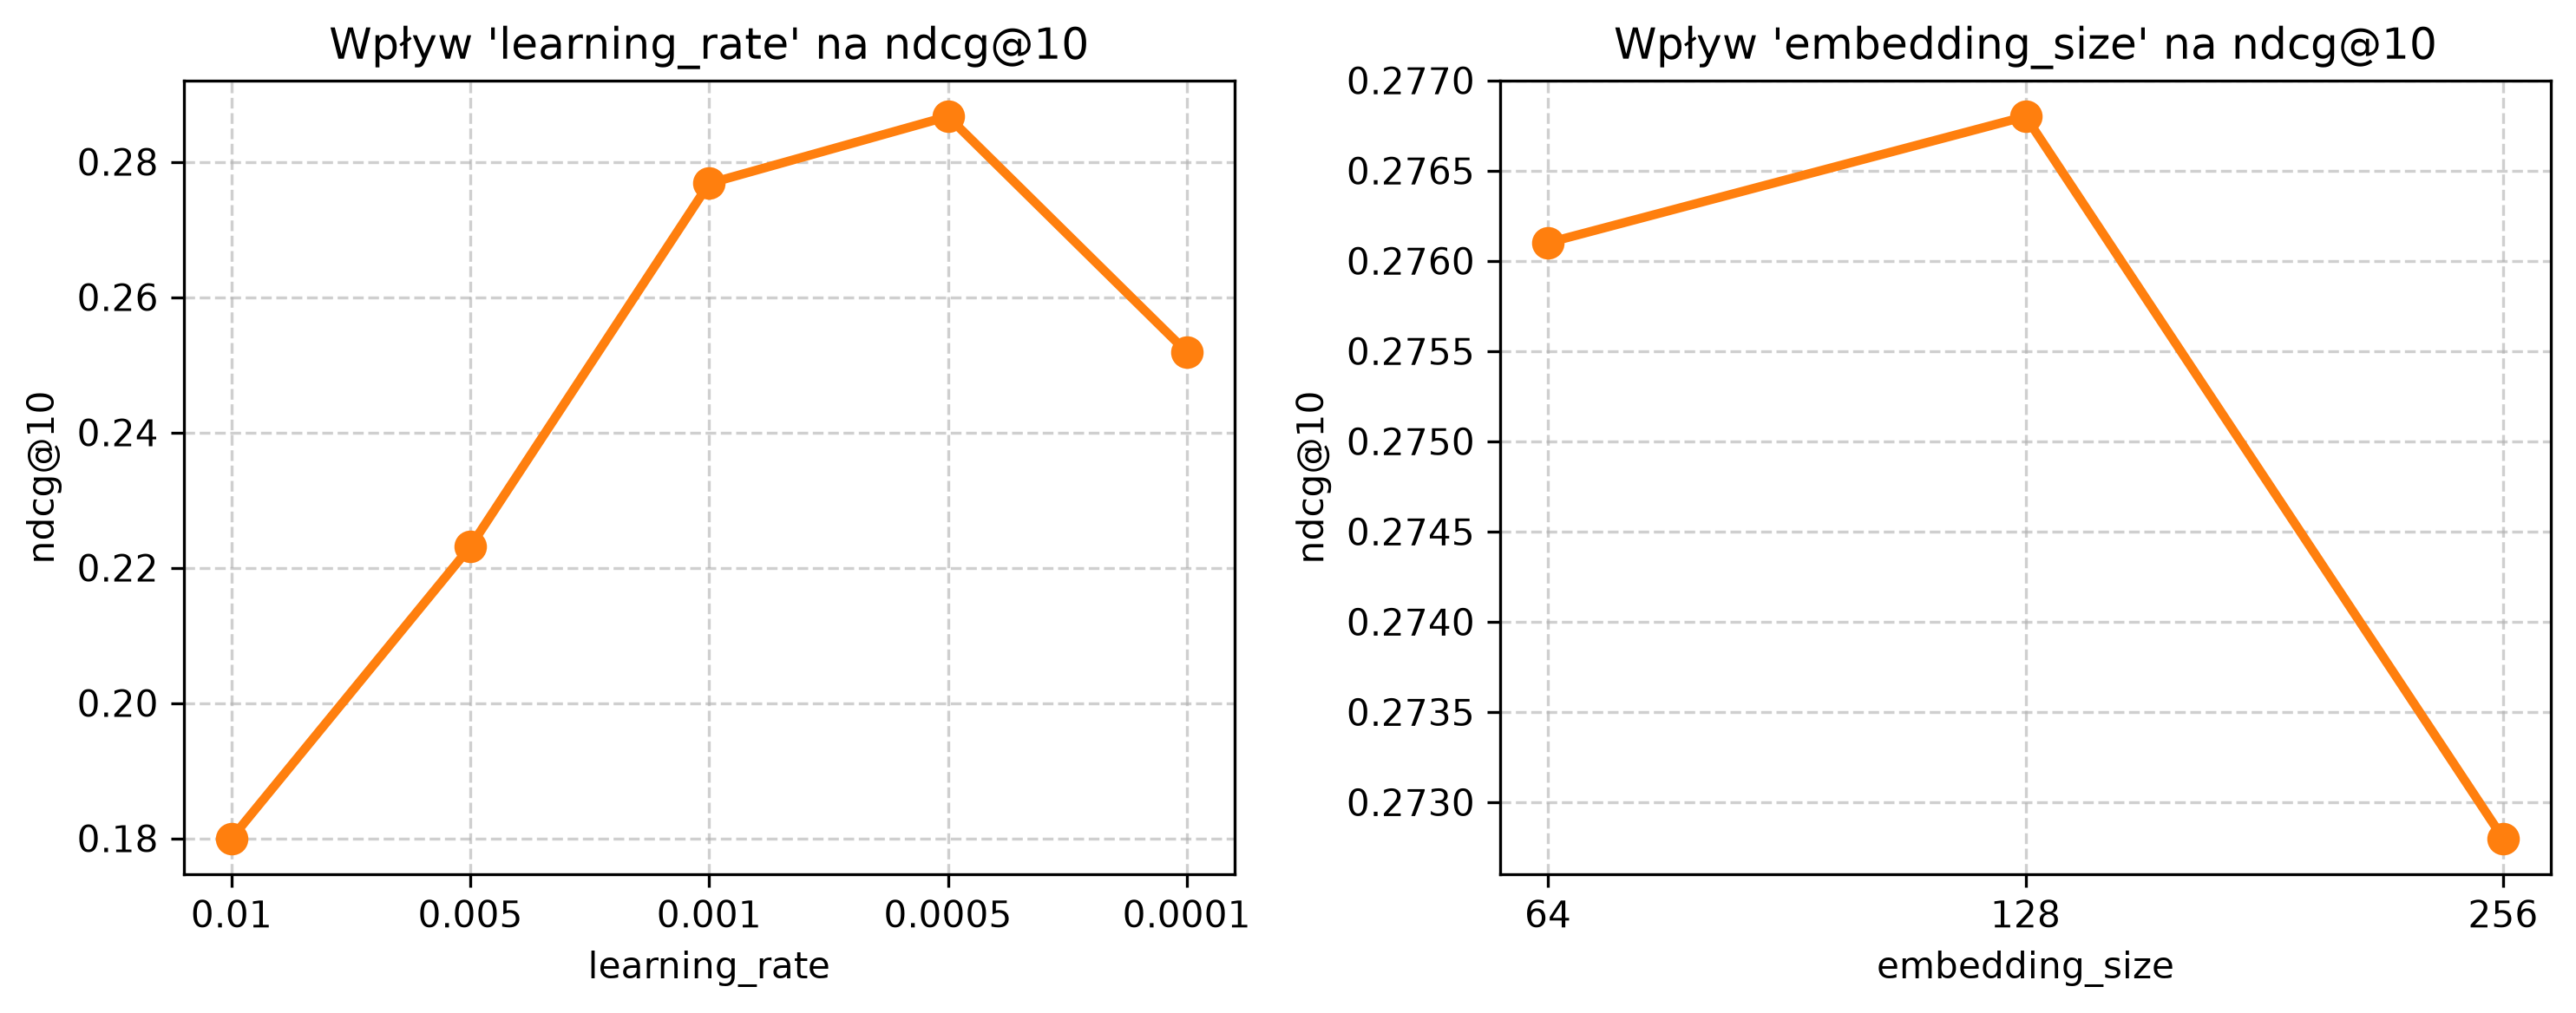
\includegraphics[width=\textwidth]{img/sweep_bpr_summary.png}
    \caption{Wpływ współczynnika uczenia oraz rozmiaru wektora zanurzeń na trafność modelu BPR}
    \label{fig:sweep_bpr}
    \vspace{0.2cm}\noindent{\raggedright \small \textbf{Źródło:} opracowanie własne.\par}
\end{figure}

Ocena parametrów hybrydowego modelu NeuMF (Rysunek \ref{fig:sweep_neumf}) potwierdza specyfikę głębokich sieci neuronowych. Widać jednoznacznie, że model zbiega do globalnego optimum przy \textit{learning rate} na poziomie 0.0001 (NDCG $\approx$ 0.2810). Parametr \textit{dropout} wykazuje z kolei wysoce czytelny punkt optymalny dla wartości 0.5. Pozwala to na odpowiednią, restrykcyjną regularyzację gęstych warstw, skutecznie hamując overfitting i zwiększając zdolność uogólniania wniosków.

\begin{figure}[H]
    \centering
    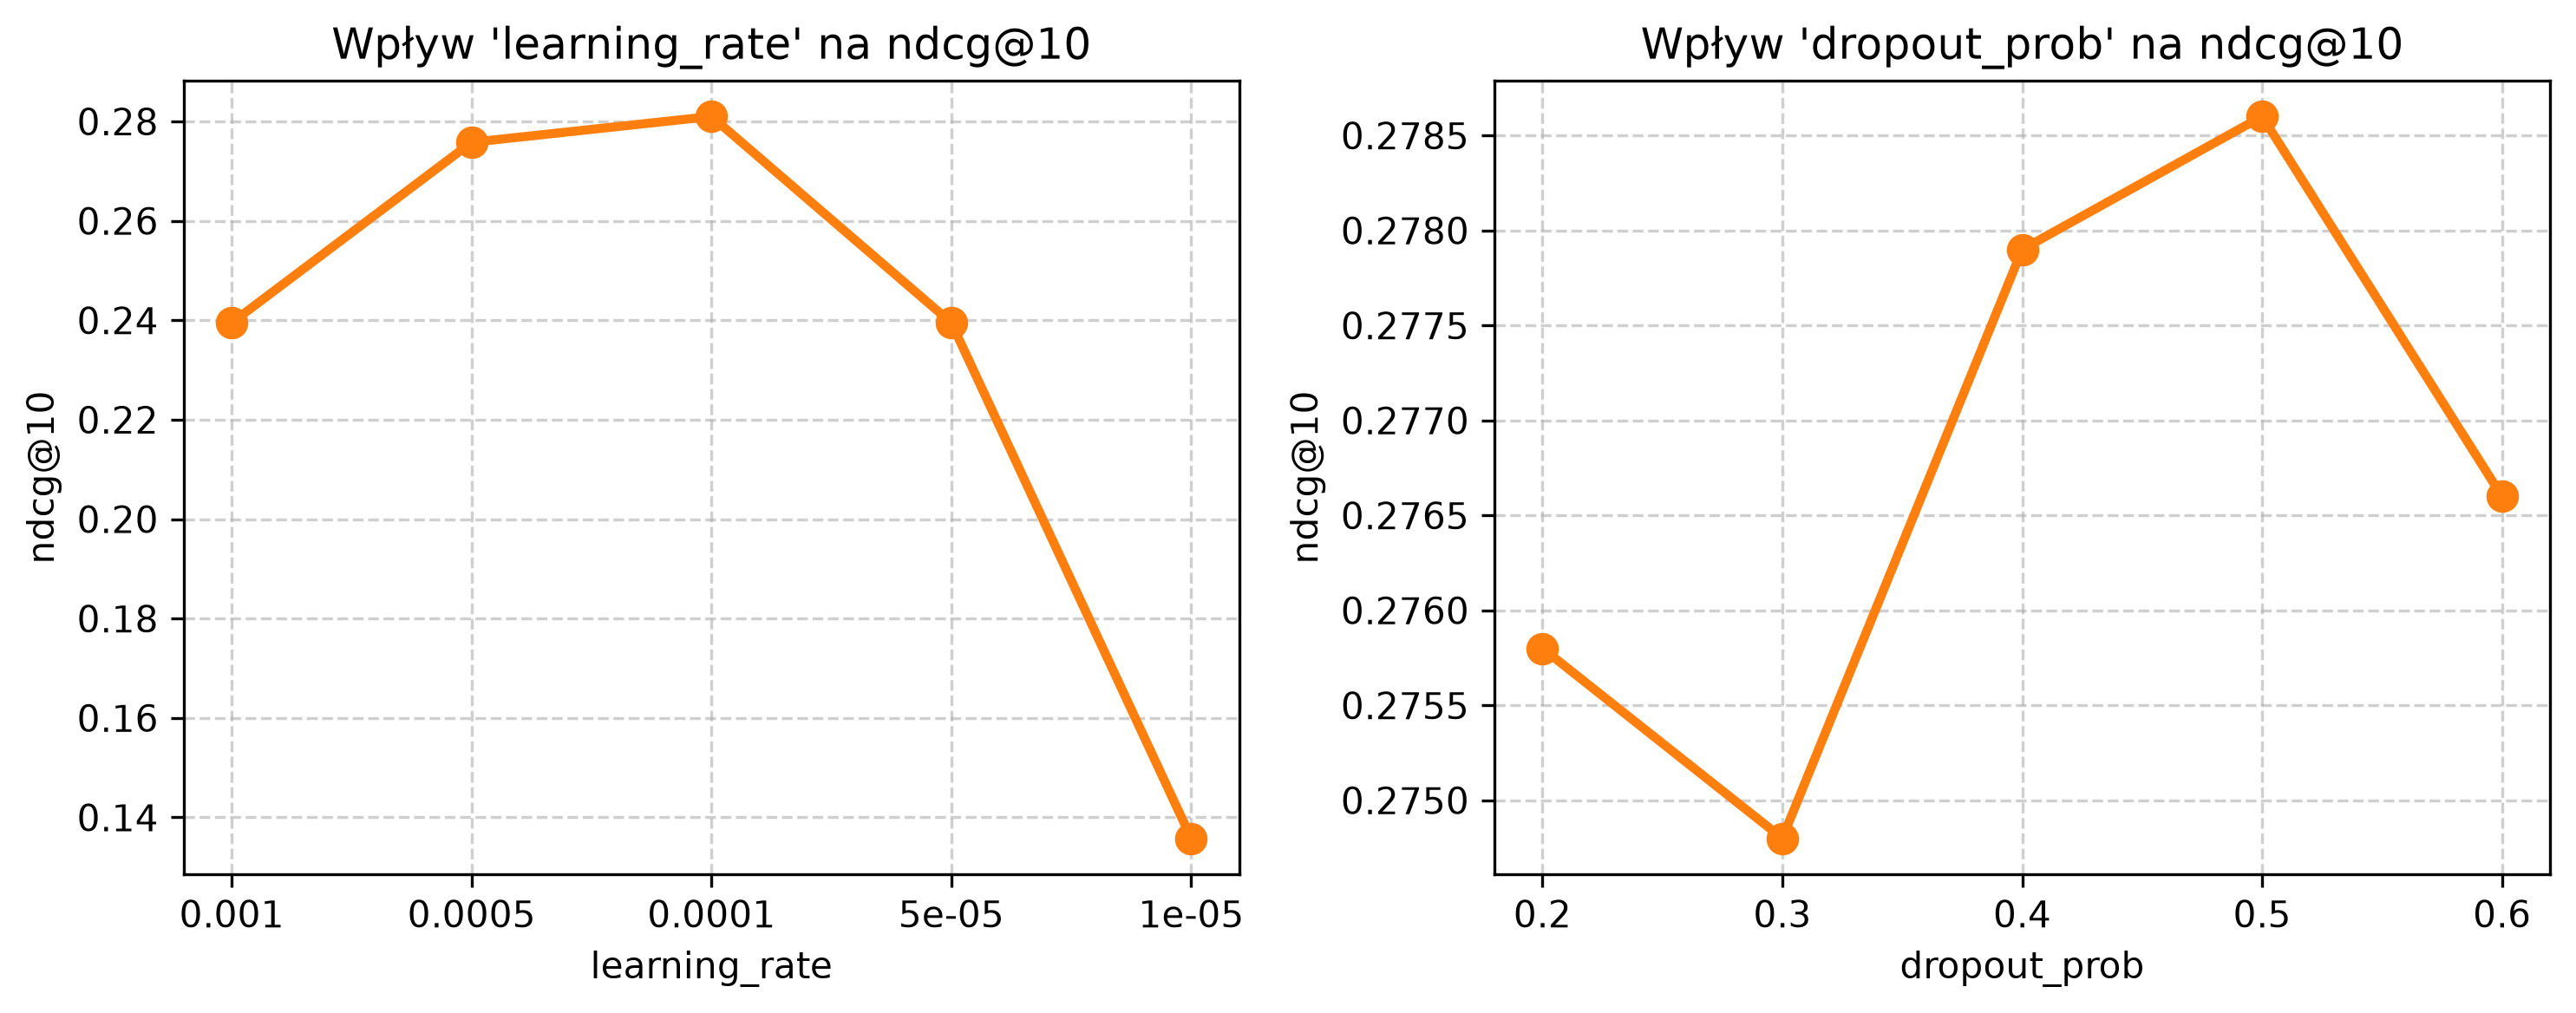
\includegraphics[width=\textwidth]{img/sweep_neumf_summary.png}
    \caption{Wpływ współczynnika uczenia oraz parametru dropout na trafność modelu NeuMF}
    \label{fig:sweep_neumf}
    \vspace{0.2cm}\noindent{\raggedright \small \textbf{Źródło:} opracowanie własne.\par}
\end{figure}

Ostatnim etapem analizy była ocena grafowego modelu LightGCN (Rysunek \ref{fig:sweep_lightgcn}). Architektura ta bazuje na propagacji informacji wzdłuż krawędzi, co ma swoje odzwierciedlenie na wykresie: zastosowanie dwóch warstw propagacji (\textit{n\_layers = 2}) okazało się optymalne. Zwiększanie liczby warstw do 3 lub 4 nieznacznie pogarsza wyniki, co jest klasycznym objawem problemu nadmiernego wygładzenia sygnałów (ang. \foreignlanguage{english}{\textit{over-smoothing}}). Zastosowanie odpowiedniej siły kary za wielkość wag również posiada ostry szczyt użyteczności: \textit{reg\_weight = 0.10} maksymalizuje końcową precyzję predykcji tego algorytmu.

\begin{figure}[H]
    \centering
    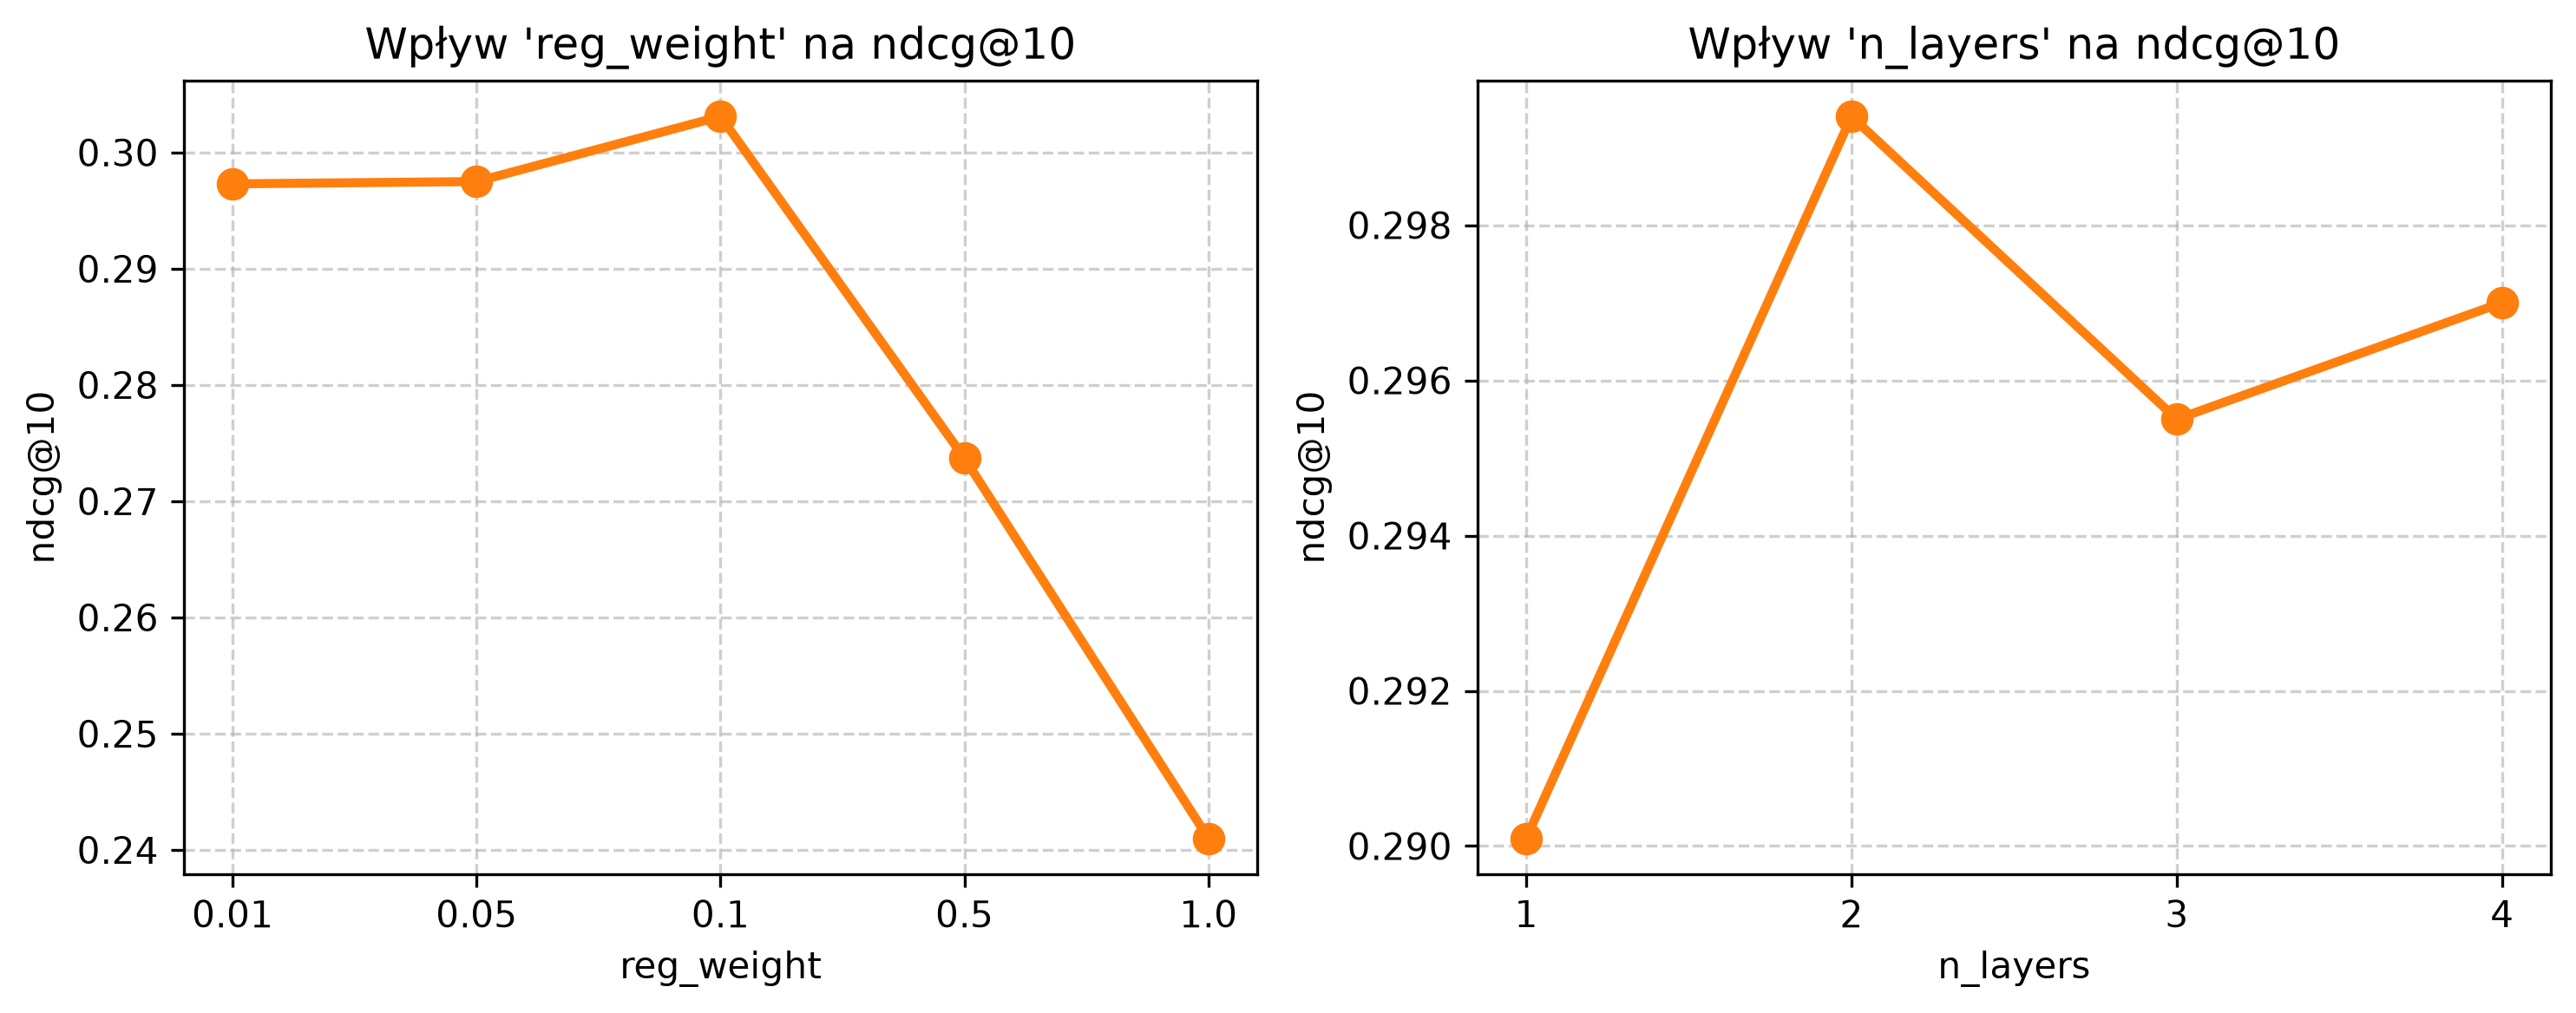
\includegraphics[width=\textwidth]{img/sweep_lightgcn_summary.png}
    \caption{Wpływ wagi regularyzacji oraz liczby warstw propagacji na trafność modelu LightGCN}
    \label{fig:sweep_lightgcn}
    \vspace{0.2cm}\noindent{\raggedright \small \textbf{Źródło:} opracowanie własne.\par}
\end{figure}


\subsubsection{Przeszukiwanie siatki parametrów --- Grid Search}

Do ostatecznej optymalizacji hiperparametrów wykorzystano metodę przeszukiwania siatki (\textit{Grid Search}). Jest to podejście deterministyczne, w którym dla każdego badanego parametru definiuje się dyskretny zbiór wartości, a następnie sprawdza każdą możliwą ich kombinację. Złożoność obliczeniowa tego procesu rośnie wykładniczo wraz z liczbą analizowanych wymiarów, co w naturalny sposób narzuca konieczność wcześniejszej redukcji przestrzeni wariantów.

Dzięki przeprowadzonej wcześniej, szczegółowej analizie wrażliwości (Sekcja 3.1.1) udało się odrzucić nieperspektywiczne przedziały wartości i drastycznie zawęzić ostateczną przestrzeń poszukiwań. Pozwoliło to na bezpieczne wykorzystanie metody \textit{Grid Search}, która w przeciwieństwie do podejść stochastycznych (takich jak \foreignlanguage{english}{\textit{Random Search}}) gwarantuje bezwzględne odnalezienie globalnego optimum w obrębie zadanej siatki. Opierając się na wytycznych z analizy, dla każdego algorytmu zdefiniowano okrojoną przestrzeń hiperparametrów, którą zestawiono w Tabeli \ref{tab:grid_search_space}. Zgodnie z metodologią badawczą, dla każdej możliwej konfiguracji zdefiniowanej w siatce inicjowano całkowicie niezależny proces uczenia od podstaw. Ewaluacja poszczególnych wariantów odbywała się wyłącznie na wyodrębnionym zbiorze walidacyjnym, co pozwalało na obiektywny wybór modelu i chroniło finalny zbiór testowy przed zjawiskiem przedwczesnego dopasowania. Za ostateczne kryterium wyboru najlepszego zestawu hiperparametrów przyjęto maksymalizację metryki NDCG@10.

Warto w tym miejscu zaznaczyć, że współczesne algorytmy rekomendacyjne -- w szczególności te oparte na sieciach neuronowych -- charakteryzują się rozbudowaną przestrzenią konfiguracyjną. Jednoczesna optymalizacja wszystkich dostępnych hiperparametrów przy użyciu metody \textit{Grid Search} była niemożliwa ze względu na wykładniczy wzrost czasu trwania obliczeń. Z tego powodu proces strojenia świadomie ograniczono wyłącznie do kluczowych parametrów, zidentyfikowanych w analizie wrażliwości jako najbardziej wpływowe dla poszczególnych architektur.

Zdecydowana większość pozostałych ustawień procesu uczenia, niewyszczególnionych w Tabeli \ref{tab:grid_search_space}, została ustandaryzowana i zachowana na stałym poziomie dla badanych algorytmów. Do aktualizacji wag wykorzystano optymalizator Adam, będący powszechnie uznanym standardem w środowisku RecBole. Rozmiar partii danych ustalono na 4096, co zapewniło odpowiednią stabilność numeryczną gradientu. Maksymalną liczbę iteracji ograniczono do 100 epok, z włączonym mechanizmem wczesnego zatrzymywania -- trening przerywano, gdy metryka NDCG@10 na zbiorze walidacyjnym nie uległa poprawie przez 10 kolejnych epok. Strategię negatywnego próbkowania uzależniono z kolei od specyfiki optymalizacji. Algorytmy bazujące na parowej funkcji straty BPR (klasyczny BPR oraz LightGCN) trenowano w schemacie 1:1, parując każdą interakcję pozytywną z jedną losową interakcją negatywną. Z kolei model NeuMF, zoptymalizowany pod kątem straty punktowej, trenowano stosując proporcję 1:4 (cztery próbki negatywne na jedną obserwowaną). Odpowiednie dostosowanie tego aspektu do natywnych mechanizmów poszczególnych architektur gwarantuje, że końcowa ewaluacja w pełni oddaje ich faktyczny potencjał.

\begin{table}[H]
    \centering
    \caption{Zestawienie przestrzeni hiperparametrów (siatki) dla poszczególnych algorytmów}
    \label{tab:grid_search_space}
    \begin{tabular}{|l|l|l|}
    \hline
    \textbf{Model}            & \textbf{Parametr}        & \textbf{Przestrzeń poszukiwań (Grid)} \\ \hline
    \multirow{2}{*}{ItemKNN}  & $k$                      & \{100, 150, 200\}                     \\ \cline{2-3}
                              & \textit{shrink}          & \{0.0, 2.5, 5.0, 7.5, 10.0\}          \\ \hline
    \multirow{2}{*}{BPR}      & \textit{learning\_rate}  & \{0.001, 0.0005, 0.0001\}             \\ \cline{2-3}
                              & \textit{embedding\_size} & \{64, 128\}                           \\ \hline
    \multirow{2}{*}{NeuMF}    & \textit{learning\_rate}  & \{0.0005, 0.0001, 0.00005\}           \\ \cline{2-3}
                              & \textit{dropout\_prob}   & \{0.4, 0.5, 0.6\}                     \\ \hline
    \multirow{2}{*}{LightGCN} & \textit{reg\_weight}     & \{0.01, 0.05, 0.1\}                   \\ \cline{2-3}
                              & \textit{n\_layers}       & \{2, 4\}                              \\ \hline
\end{tabular}


    \vspace{0.2cm}\noindent{\raggedright \small \textbf{Źródło:} opracowanie własne.\par}
\end{table}

Wyniki procesu optymalizacji pozwoliły na wyłonienie ostatecznych architektur, które posłużą do finalnego porównania skuteczności algorytmów w kolejnym podrozdziale. Zestawienie wyselekcjonowanych parametrów przedstawiono w Tabeli \ref{tab:finalne_parametry}:
\begin{itemize}
    \item \textbf{ItemKNN}: Najlepszą celność uzyskano dla sąsiedztwa $k=100$ oraz wygładzania \textit{shrinkage} $= 7.5$ (NDCG@10 $= 0.2734$).
    \item \textbf{BPR}: Wariant z optymalizacją bayesowską najlepiej operował w przestrzeni latentnej o rozmiarze $128$ przy kroku uczenia równym $0.001$ (NDCG@10 $= 0.2837$).
    \item \textbf{NeuMF}: Algorytm oparty na głębokich sieciach neuronowych osiągnął globalne optimum dla współczynnika odrzucenia (dropout) rzędu $0.5$ oraz współczynnika uczenia $0.0005$ (NDCG@10 $= 0.2895$). Pozostałe, stałe parametry architektoniczne (w tym rozmiary warstw ukrytych) zostały zachowane na podstawie wcześniejszej analizy.
    \item \textbf{LightGCN}: Model grafowy zdominował zestawienie testowe, uzyskując najwyższą bezwzględną trafność (NDCG@10 $= 0.3021$) dla $2$ warstw propagacji wzdłuż krawędzi oraz wagi regularyzacji L2 na poziomie $0.1$.
\end{itemize}

Powyższe zestawy parametrów gwarantują, że podczas ostatecznej ewaluacji każdy z modeli będzie operował na możliwie najlepiej dobranych wartościach i osiągał optymalne wyniki.

\begin{table}[H]
    \centering
    \caption{Wyselekcjonowane, optymalne wartości hiperparametrów dla badanych modeli}
    \label{tab:finalne_parametry}
    \begin{tabular}{|l|l|c|}
    \hline
    \textbf{Model} & \textbf{Parametr} & \textbf{Optymalna wartość} \\ \hline
    \multirow{2}{*}{ItemKNN}  & $k$ & 100 \\ \cline{2-3}
                              & \textit{shrink} & 7.5 \\ \hline
    \multirow{2}{*}{BPR}      & \textit{learning\_rate} & 0.001 \\ \cline{2-3}
                              & \textit{embedding\_size} & 128 \\ \hline
    \multirow{2}{*}{NeuMF}    & \textit{learning\_rate} & 0.0005 \\ \cline{2-3}
                              & \textit{dropout\_prob} & 0.5 \\ \hline
    \multirow{2}{*}{LightGCN} & \textit{reg\_weight} & 0.1 \\ \cline{2-3}
                              & \textit{n\_layers} & 2 \\ \hline
\end{tabular}


    \vspace{0.2cm}\noindent{\raggedright \small \textbf{Źródło:} opracowanie własne.\par}
\end{table}

\subsection{Wyniki badań}

W niniejszym podrozdziale zaprezentowano ostateczne zestawienie skuteczności badanych algorytmów. Ocenę przeprowadzono na odseparowanym zbiorze testowym, gwarantując tym samym obiektywną miarę zdolności modeli do generalizacji. Zgodnie z wcześniej przyjętą metodologią, predykcje poszczególnych architektur oceniono z wykorzystaniem metryk NDCG@10, Recall@10, HR@10 oraz MRR@10. Pełne zestawienie wyników zaprezentowano w Tabeli \ref{tab:wyniki_eksperymentow}.

\begin{table}[H]
    \centering
    \caption{Porównanie wyników metryk oceny dla testowanych algorytmów rekomendacyjnych na zbiorze MovieLens 100K.}
    \label{tab:wyniki_eksperymentow}
    \begin{tabular}{|l|c|c|c|c|}
\hline
\textbf{Model} & \textbf{NDCG@10} & \textbf{Recall@10} & \textbf{Hit@10} & \textbf{MRR@10} \\ \hline
ItemKNN & 0.2734 & 0.2336 & 0.7497 & 0.4392 \\ \hline
BPR & 0.2837 & \underline{0.2437} & 0.7603 & 0.4525 \\ \hline
NeuMF & \underline{0.2895} & 0.2435 & \textbf{0.7720} & \underline{0.4744} \\ \hline
LightGCN & \textbf{0.3021} & \textbf{0.2529} & \underline{0.7678} & \textbf{0.4835} \\ \hline
\end{tabular}

    \vspace{0.2cm}\noindent{\raggedright \small \textbf{Źródło:} opracowanie własne.\par}
\end{table}

Analiza powyższej tabeli pozwala na wyciągnięcie kilku kluczowych wniosków, które wpisują się w historyczną ewolucję systemów rekomendacyjnych. Punktem odniesienia w eksperymencie był najprostszy algorytm oparty na sąsiedztwie -- ItemKNN, który uzyskał najniższe, bazowe wyniki. Wprowadzenie klasycznej faktoryzacji macierzy (BPR) znacząco poprawiło jakość rekomendacji (wzrost NDCG z 0.2734 na 0.2837), co dowodzi wyższości uczenia się cech ukrytych nad prostymi heurystykami podobieństwa.

Wykorzystanie głębokich sieci neuronowych w modelu NeuMF przyniosło dalszą poprawę w większości metryk, jednak na szczególną uwagę zasługuje relacja między wskaźnikami HR@10 a NDCG@10. Choć NeuMF wygrał w kategorii HR@10 (0.7720), co oznacza, że skuteczniej umieszczał przynajmniej jeden trafny element w pierwszej dziesiątce, to ustąpił w rankingu NDCG. Dowodzi to, że osiągający najwyższe wyniki w zestawieniu grafowy model LightGCN znacznie lepiej radzi sobie z precyzyjnym pozycjonowaniem trafnych rekomendacji na samym szczycie listy. Architektura grafowa, dzięki jawnej propagacji sygnałów między użytkownikami a przedmiotami, uzyskała najwyższe wartości NDCG@10 (0.3021) oraz MRR@10 (0.4835).

\subsubsection{Krzywe zbieżności i stabilność procesu uczenia}

Zestawienie końcowych wyników uzupełniono o analizę dynamiki procesu uczenia poszczególnych architektur. Na Rysunku \ref{fig:learning_curves} zaprezentowano krzywe zbieżności (ang. \foreignlanguage{english}{\textit{learning curves}}) rejestrujące zmianę metryki NDCG@10 na zbiorze walidacyjnym w trakcie trwania optymalizacji, aż do momentu aktywacji mechanizmu wczesnego zatrzymywania.

\begin{figure}[H]
    \centering
    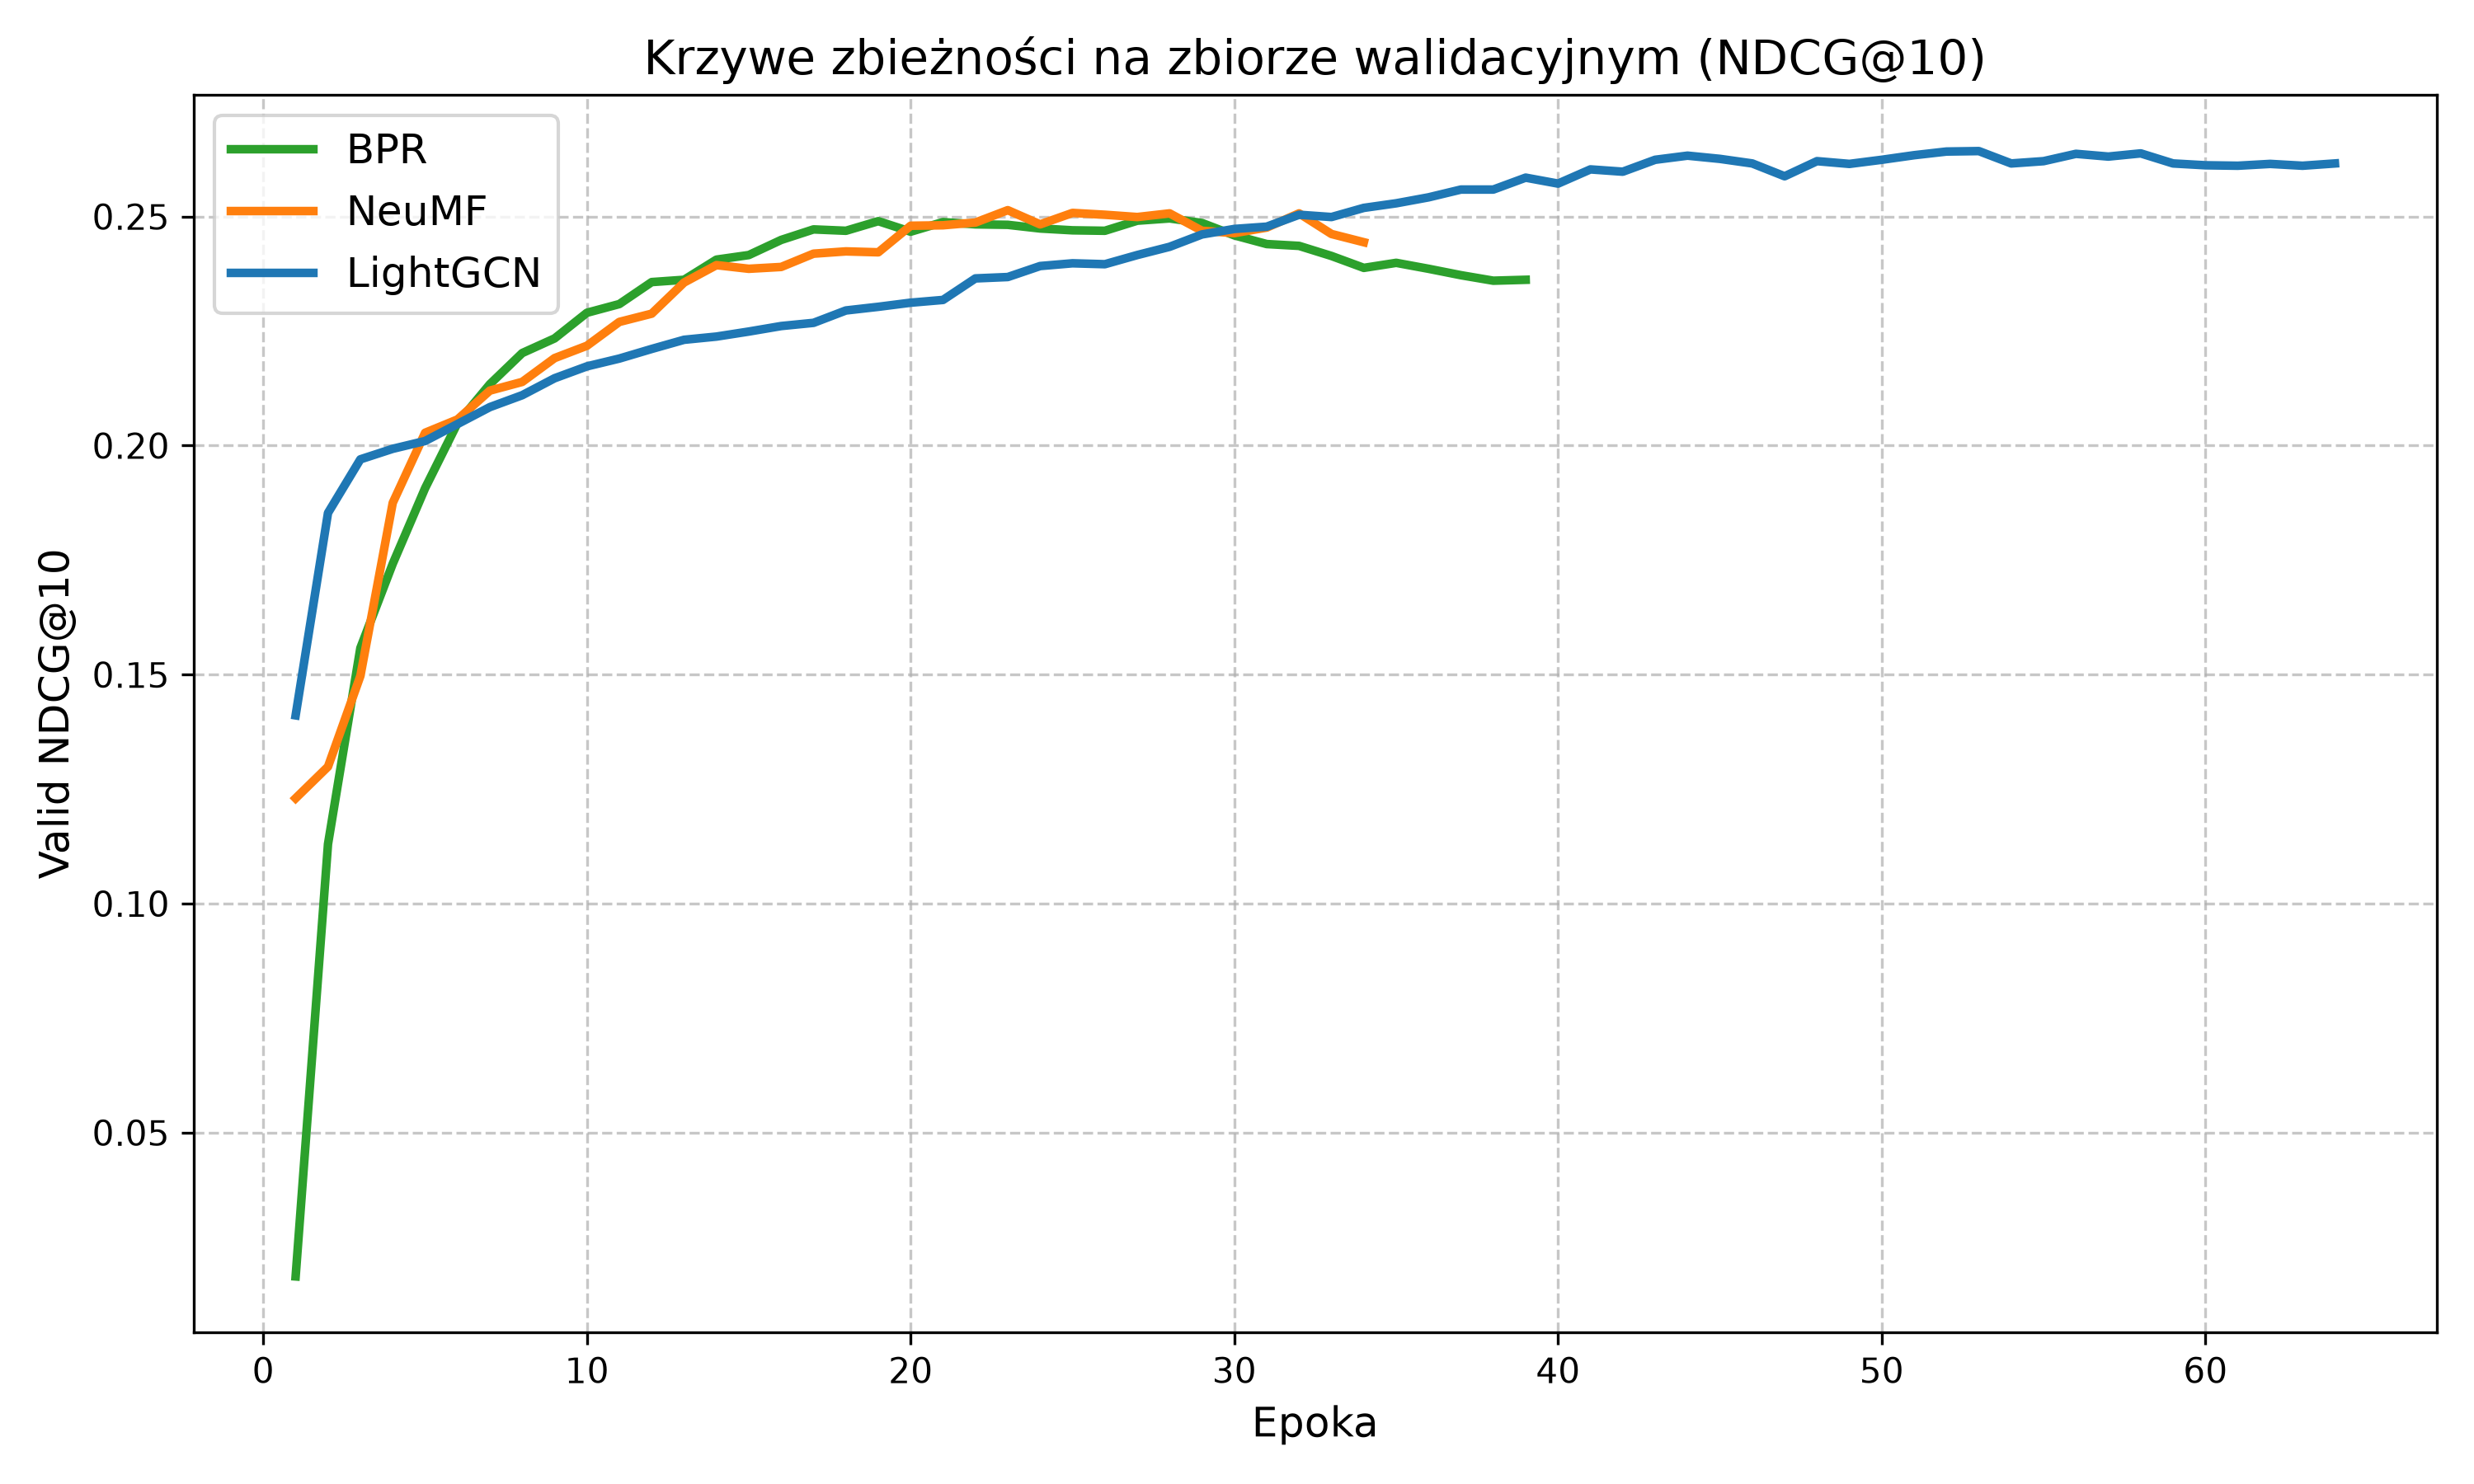
\includegraphics[width=0.85\textwidth]{img/learning_curves.png}
    \caption{Krzywe zbieżności metryki NDCG@10 na zbiorze walidacyjnym dla algorytmów BPR, NeuMF oraz LightGCN.}
    \label{fig:learning_curves}
    \vspace{0.2cm}\noindent{\raggedright \small \textbf{Źródło:} opracowanie własne.\par}
\end{figure}

Analiza krzywych ujawnia interesujące różnice w sposobie optymalizacji. Klasyczny model faktoryzacji macierzy (BPR) wykazuje najszybsze tempo zbieżności -- jego trafność gwałtownie rośnie już w pierwszych iteracjach, osiągając lokalne optimum w okolicach 20. epoki. Następnie można zaobserwować delikatny spadek jakości, co świadczy o podatności na przeuczenie na zbiorze treningowym. Z kolei model grafowy (LightGCN) startuje z niższego poziomu i uczy się znacznie wolniej, jednak jego krzywa jest wysoce stabilna. Ostatecznie, proces powolnego propagowania sygnałów w grafie pozwala na przekroczenie pułapu wyznaczonego przez BPR i NeuMF, a optymalna zbieżność osiągana jest znacznie później.

\subsubsection{Koszty obliczeniowe a skuteczność algorytmów}

Ostatnim elementem ewaluacji jest analiza relacji nakładów obliczeniowych (czasu optymalizacji modelu) do uzyskiwanej trafności predykcji. Jest to kluczowy wskaźnik inżynieryjny w środowiskach produkcyjnych, w których systemy rekomendacyjne muszą być regularnie i szybko dotrenowywane nowymi danymi. Zależność tę zilustrowano na Rysunku \ref{fig:time_vs_ndcg}.

\begin{figure}[H]
    \centering
    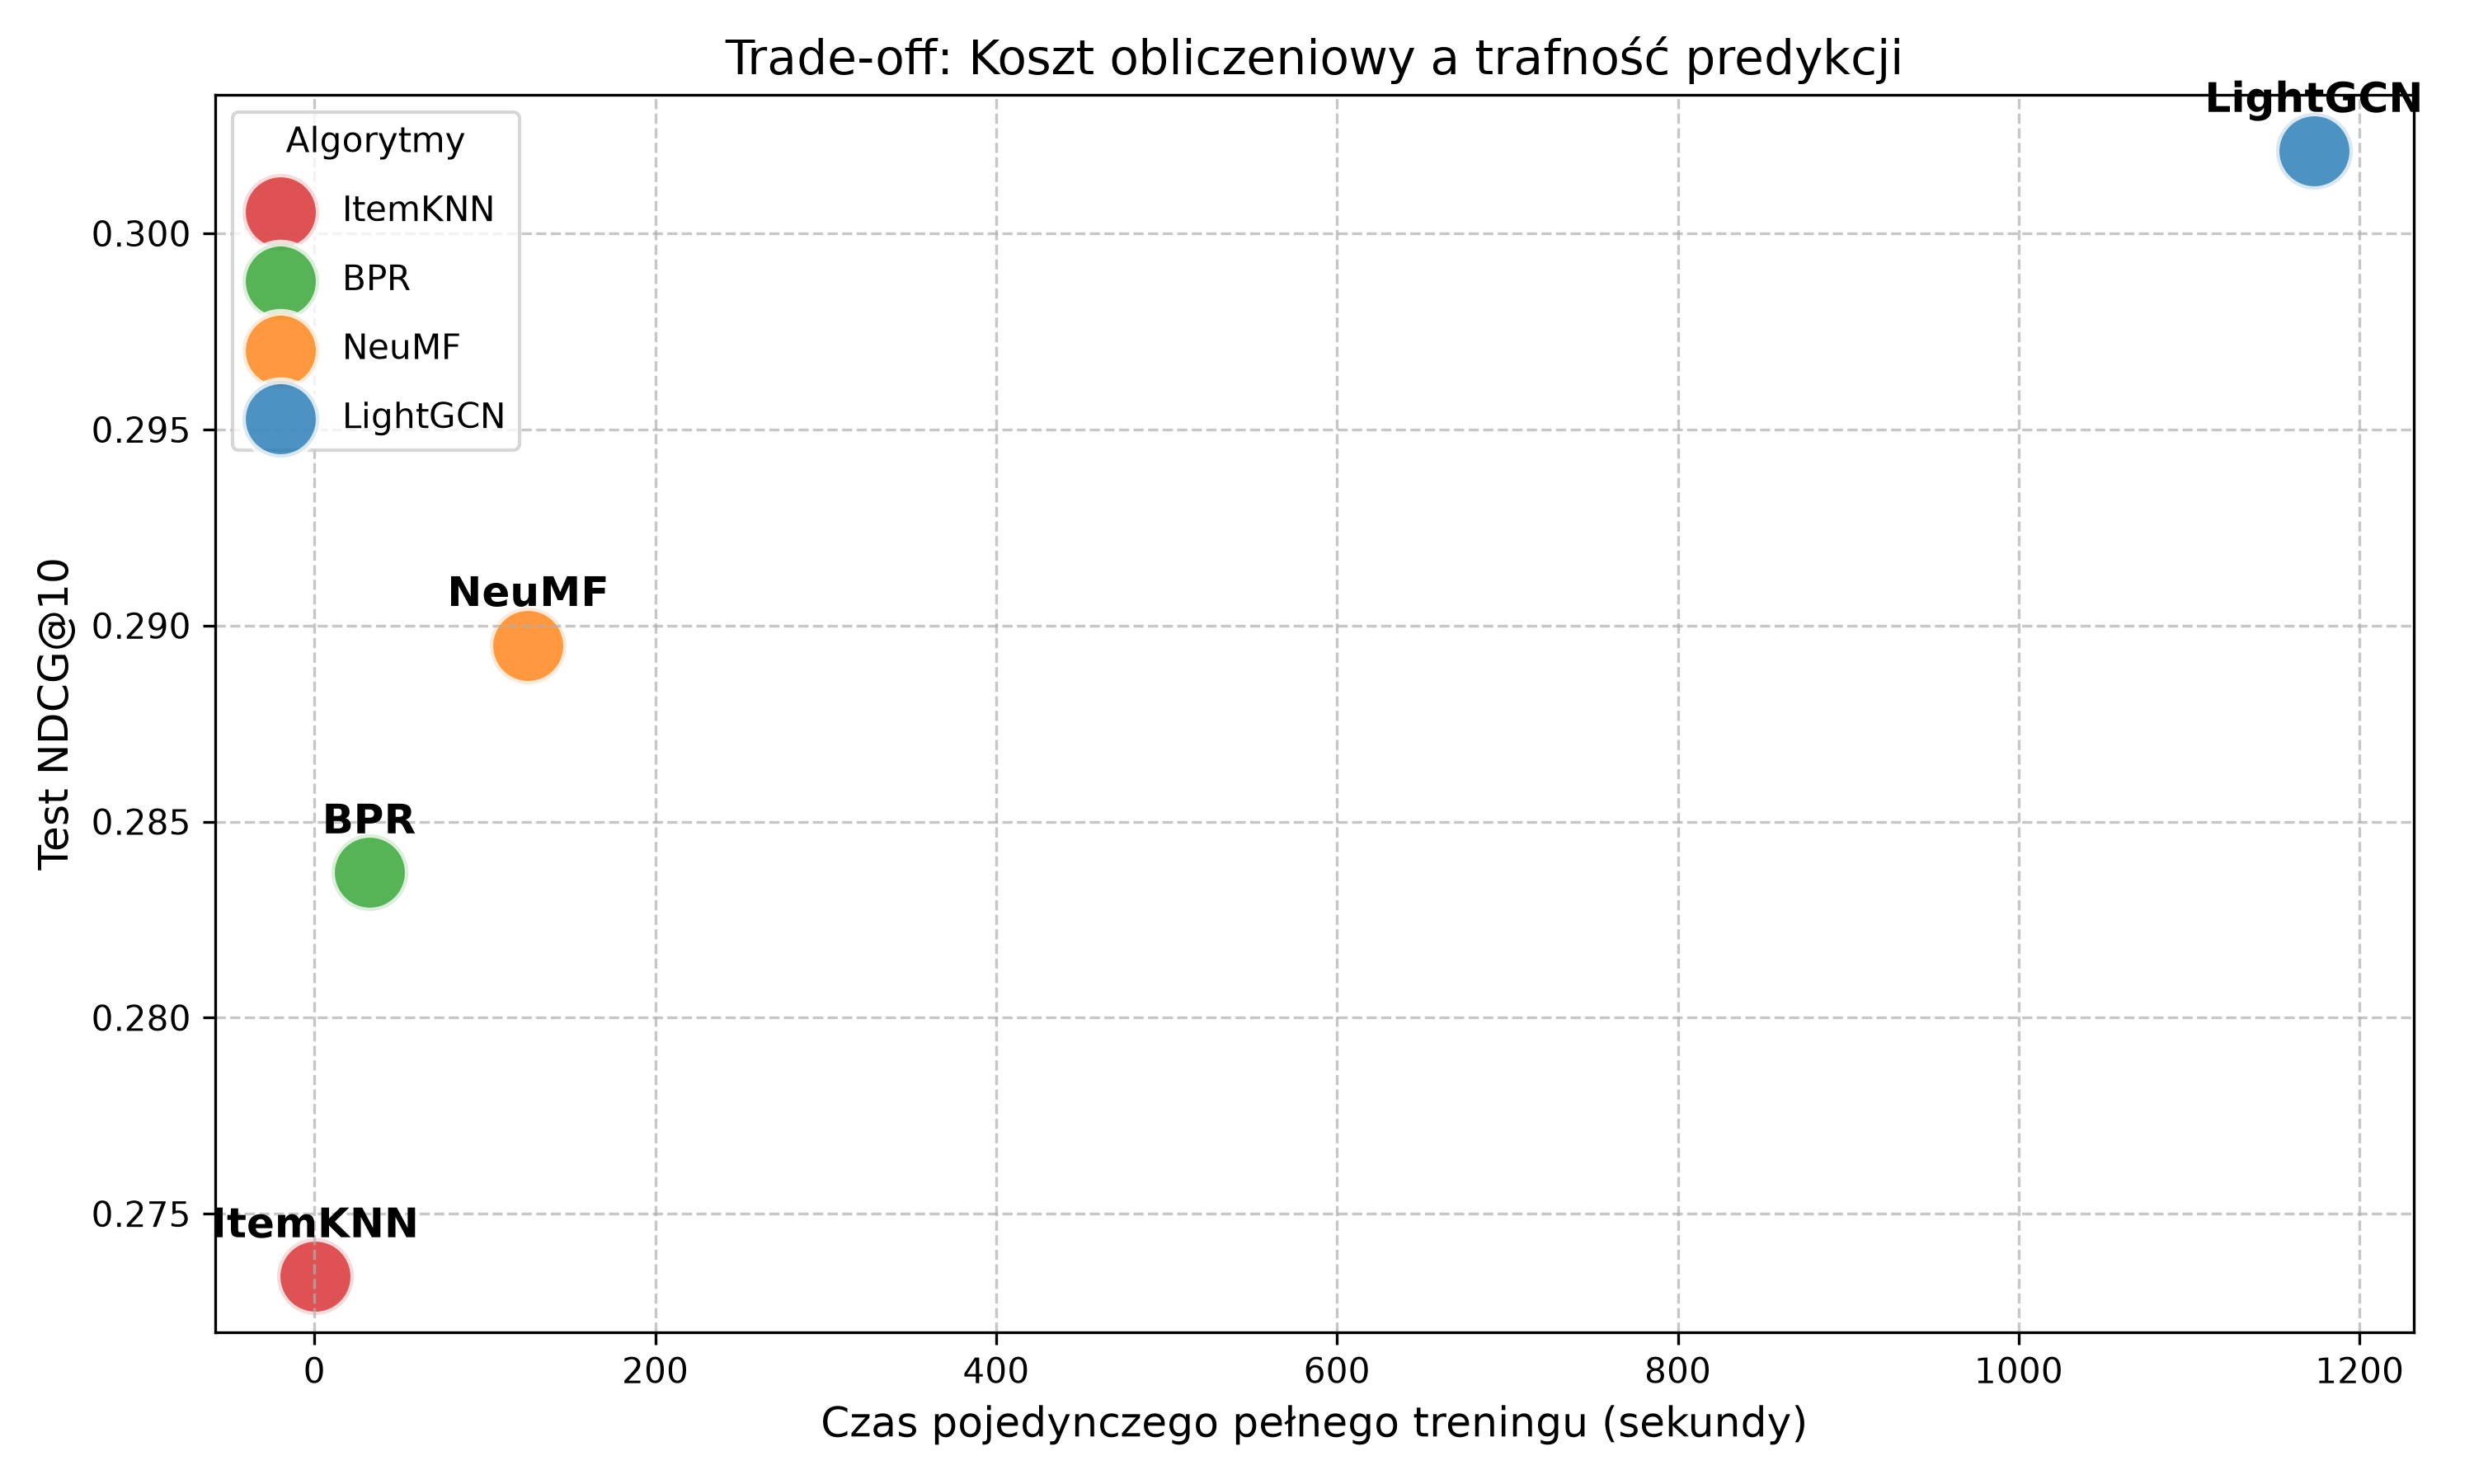
\includegraphics[width=0.8\textwidth]{img/time_vs_ndcg.png}
    \caption[Zestawienie czasu uczenia względem ostatecznej skuteczności dla badanych modeli.]{Zestawienie czasu uczenia względem ostatecznej skuteczności (NDCG@10) dla badanych modeli.}
    \label{fig:time_vs_ndcg}
    \vspace{0.2cm}\noindent{\raggedright \small \textbf{Źródło:} opracowanie własne.\par}
\end{figure}

Wykres punktowy ukazuje bardzo wyraźny kompromis pomiędzy kosztem a jakością. Model bazowy ItemKNN, nie wymagający iteracyjnej optymalizacji stochastycznej, zapewnia bardzo krótki czas odpowiedzi przy relatywnie najniższej skuteczności. Klasyczny wariant BPR jawi się jako algorytm niezwykle efektywny kosztowo. Czas jego uczenia zamyka się w kilkudziesięciu sekundach, dostarczając bardzo zadowalające rezultaty.

Najważniejszym wnioskiem jest jednak ewaluacja grafowych sieci neuronowych. Choć LightGCN przewyższa pozostałe modele pod kątem metryki NDCG, to odbywa się to znacznym kosztem sprzętowym. Czas jego pełnego treningu okazał się niemal 10-krotnie wyższy niż w przypadku głębokiej sieci neuronowej (NeuMF) oraz rzędy wielkości wyższy w porównaniu do klasycznej faktoryzacji macierzy. Wynik ten wskazuje na potencjalne ograniczenia wdrożeniowe algorytmu w czasie rzeczywistym.

\subsection{Dyskusja wyników i wnioski}

Przeprowadzone badania eksperymentalne na zbiorze MovieLens 100K dostarczyły dowodów na to, że ewolucja systemów rekomendacyjnych w kierunku architektur uwzględniających szerszy kontekst powiązań pomiędzy obiektami jest kierunkiem gwarantującym stosunkowo najlepsze wyniki. Metryki rangowe potwierdziły teoretyczną hierarchię modeli, układając się w czytelny ciąg rosnącej skuteczności: od najprostszych metod opartych na pamięci (ItemKNN), poprzez klasyczną faktoryzację macierzy (BPR), głębokie sieci neuronowe (NeuMF), aż po grafowe sieci neuronowe (LightGCN).

Zwycięstwo algorytmu LightGCN we wskaźnikach uwzględniających pozycje w rankingu (NDCG@10 na poziomie 0.3021 oraz MRR@10 wynoszące 0.4835) bezpośrednio udowadnia, że jawne włączenie struktury grafu dwudzielnego do procesu uczenia pozwala na najtrafniejsze ułożenie samej czołówki listy rekomendacji. Jest to zjawisko wysoce pożądane w systemach VOD, gdzie uwaga widza skupia się na pierwszych kilku propozycjach wyświetlanych na ekranie telewizora. Interesującą obserwacją okazał się jednak wynik wskaźnika HR@10, w którym to głęboka architektura NeuMF (0.7720) zdołała nieznacznie wyprzedzić wariant grafowy (0.7678). Sugeruje to, że nieliniowe sieci wielowarstwowe wykazują zdolność do odnajdywania jakiegokolwiek trafnego obiektu i wyprowadzania go do pierwszej dziesiątki, jednak brakuje im precyzji strukturalnej (którą posiada LightGCN), aby wywindować obiekt na wyższe miejsce w rankingu.

Z inżynieryjnego i biznesowego punktu widzenia ostateczne wnioski z badań nie są jednak tak jednoznaczne, jak wskazywałyby na to same miary trafności. Analiza relacji kosztów do jakości (zob. Rysunek \ref{fig:time_vs_ndcg}) pokazała, że zastosowanie najnowocześniejszych rozwiązań opartych na propagacji wiadomości w grafie powoduje znaczny wzrost czasu uczenia. Fakt, iż trening modelu LightGCN wymagał nieporównywalnie więcej nakładów niż optymalizacja wariantu NeuMF, a tym bardziej klasycznego BPR, stanowi zauważalną barierę wdrożeniową. Na wielkoskalowych platformach streamingowych generujących setki milionów logów dziennie proces ten może okazać się problematyczny.

Podsumowując, problematyka wyboru optymalnego algorytmu na rynku komercyjnych usług dostarczania treści wideo nie powinna sprowadzać się wyłącznie do bezwzględnego pościgu za metryką NDCG. Uzyskane wyniki eksperymentalne wskazują, że chociaż grafowe sieci neuronowe bez wątpienia dostarczają obecnie najlepsze wyniki, to w realiach ograniczonego budżetu operacyjnego, drogiej infrastruktury chmurowej oraz wymogu wysokiej responsywności, rozwiązania klasyczne, takie jak zoptymalizowane podejście parowe (BPR) lub architektury hybrydowe (NeuMF), wciąż stanowią niezwykle opłacalną alternatywę.